\begin{frame}
\frametitle{Experiments - Paired Image Translation}
\framesubtitle{Baselines}
Training details:
\begin{itemize}
    \item 330MB of trainable parameters for unpaired models(LoRA weights, zero-conv layer, first conv layer of U-Net)
    \item Adam Optimizer with learning rate: 1e-6, batch size:8, $\lambda _{\text{idt}} = 1$, $\lambda _{\text{GAN}} = 0.5$
\end{itemize}
Datasets:
\begin{table}
    \centering
    \begin{tabular}{|c|c|c|c|}
        Task & Images Source & Images Target & Dataset \\
        \hline
        Horse $\leftrightarrow$ Zebra & 939 & 1177 & ImageNet \cite{5206848}\\
        Winter $\leftrightarrow$ Summer & 854 & 1273 & Flickr \cite{zhu2020unpaired} \\
        Day $\leftrightarrow$ Night & Day subset & Night subset & BDD100k \cite{yu2020bdd100k}\\
        Clear $\leftrightarrow$ Foggy & 12454 & 572 from & BDD100k and DENSE \cite{bijelic2020seeing}
    \end{tabular}       
\end{table}
\end{frame}

\begin{frame}
    \frametitle{Experiments - Paired Image Translation}
    \framesubtitle{Baselines}
    Evaluation Protocol:
    \begin{itemize}
        \item match data distribution of target domain $\rightarrow$ FID \cite{heusel2018gans}
        \item preserve input image structure in translated output $\rightarrow$ DINO \cite{tumanyan2022splicing}
        \item Inference runtime using a single NVIDIA RTX A6000 GPU
        \item human preceptual study
    \end{itemize}
    
    
\end{frame}

% ---------- Comparison to Unpaired Methods ----------
\begin{frame}
    \frametitle{Experiments - Paired Image Translation}
    \framesubtitle{Comparison to Unpaired Methods}
    \begin{figure}
        \centering
        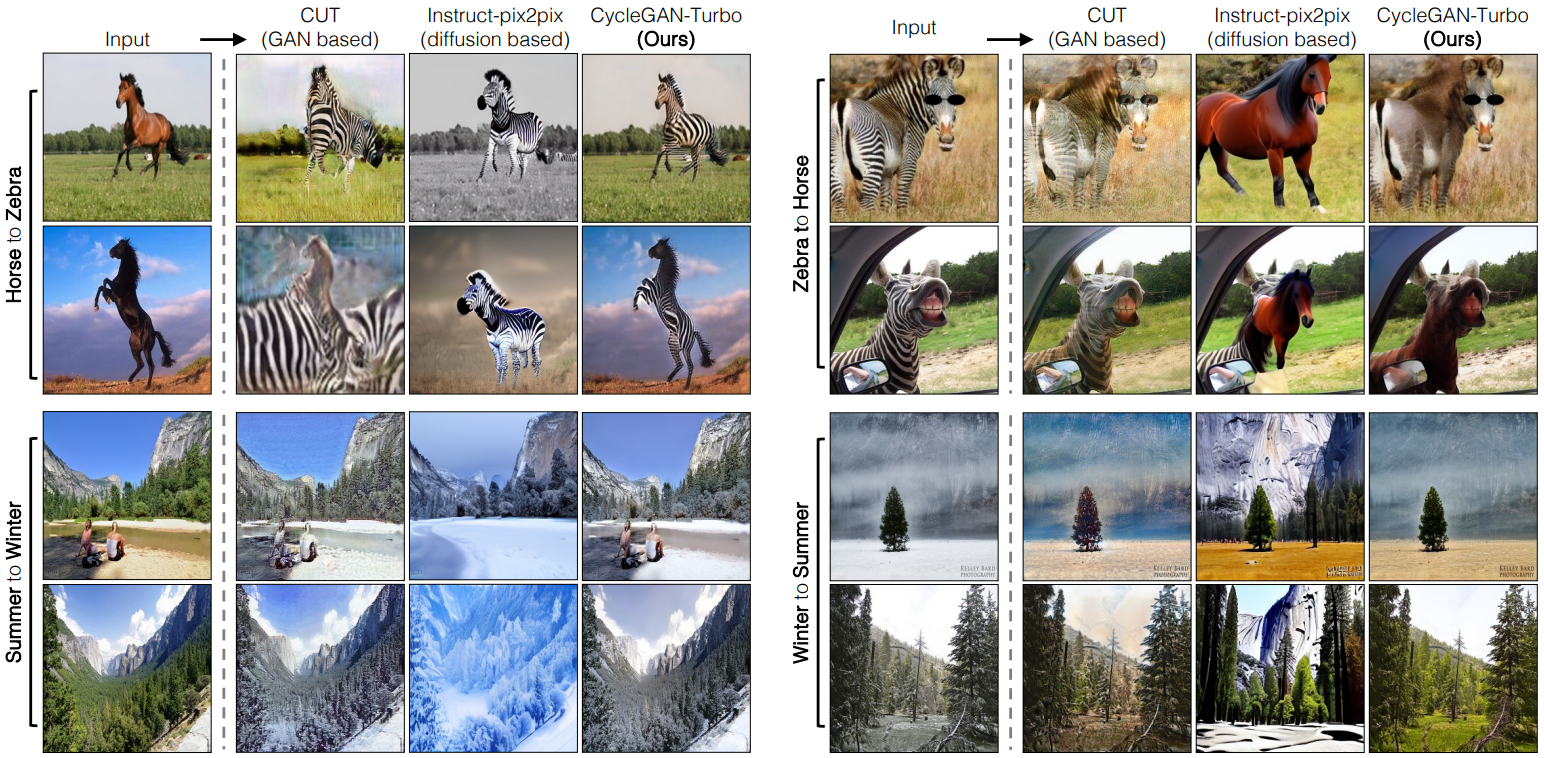
\includegraphics[width=0.85\linewidth]{images/horse_zebra.png}
        
    \end{figure}
\end{frame}


\begin{frame}
    \frametitle{Experiments - Paired Image Translation}
    \framesubtitle{Comparison to Unpaired Methods}
   
    \begin{table}
        \centering
    
     \vspace{-5pt}
        \resizebox{\linewidth}{!}{
        \begin{tabular}{l c cc cc cc cc}
            \toprule 
            \multirow{3}{*}{\textbf{Method}} 
            & \multirow{3}{*}{\textbf{\shortstack[c]{Infrence \\ time }}} 
            & \multicolumn{2}{c}{\textbf{Horse $\rightarrow$ Zebra} }
            & \multicolumn{2}{c}{\textbf{Zebra $\rightarrow$ Horse} }
            & \multicolumn{2}{c}{\textbf{Summer $\rightarrow$ Winter} }
            & \multicolumn{2}{c}{\textbf{Winter $\rightarrow$ Summer} }
            \\
    
            \cmidrule(lr){3-4} \cmidrule(lr){5-6} \cmidrule(lr){7-8} \cmidrule(lr){9-10} 
            &
            & \multirow{2}{*}{\shortstack[c]{FID $\downarrow$ }}  
            & \multirow{2}{*}{\shortstack[c]{DINO \\ Struct. $\downarrow$ }} 
    
            & \multirow{2}{*}{\shortstack[c]{FID $\downarrow$ }}  
            & \multirow{2}{*}{\shortstack[c]{DINO \\ Struct. $\downarrow$ }} 
    
            & \multirow{2}{*}{\shortstack[c]{FID $\downarrow$ }}  
            & \multirow{2}{*}{\shortstack[c]{DINO \\ Struct. $\downarrow$ }} 
    
            & \multirow{2}{*}{\shortstack[c]{FID $\downarrow$ }}  
            & \multirow{2}{*}{\shortstack[c]{DINO \\ Struct. $\downarrow$ }} 
            
            \\ \\
            \cmidrule(lr){1-10}
    
            CycleGAN \cite{zhu2020unpaired}  & 0.01s
            & 74.9 & 3.2 
            & 133.8 & 2.6
            & 62.9 & 2.6
            & 66.1 & 2.3 
            \\
            
            
            CUT \cite{park2020contrastive} & 0.01s
            & 43.9 & 6.6 
            & 186.7 & 2.5 
            & 72.1 & 2.1 
            & 68.5 & 2.1 \\
            
            \hdashline
    
            SDEdit \cite{meng2022sdedit} & 1.56s
            & 77.2 & 4.0
            & 198.5 & 4.6  
            & 66.1 & 2.1 
            & 76.9 & 2.1\\
            
            Plug\&Play \cite{tumanyan2022plugandplay} & 7.57s
            & 57.3 & 5.2  
            & 152.4 & 3.8 
            & 67.3 & 2.8 
            & 73.3 & 2.6\\
            
            Pix2Pix-Zero \cite{parmar2023zeroshot}  & 14.75s
            & 81.5 & 8.0
            & 147.4 & 7.8
            & 68.0 & 3.0
            & 93.4 & 4.3 \\
            
            Cycle-Diffusion \cite{cyclediffusion} & 3.72s
            & \textbf{38.6} & 6.0 
            & 132.5 & 5.8 
            & 64.1 & 3.6
            & 70.3 & 3.6 \\
    
            DDIB \cite{su2022dual} & 4.37s
            & 44.4 & 13.1  
            & 163.3 & 11.1 
            & 90.8 & 7.2
            & 88.9 & 6.8 \\
    
            InstructPix2Pix \cite{brooks2023instructpix2pix} & 3.86s
            & 51.0 & 6.8 
            & 141.5 & 7.0 
            & 68.3 & 3.7 
            & 85.6 & 4.4 \\
            \hdashline
    
            CycleGAN-Turbo & 0.13s
            & 41.0 & \textbf{2.1}
            & \textbf{127.5} & \textbf{1.8} 
            & \textbf{56.3} & \textbf{0.6} 
            & \textbf{60.7} & \textbf{0.6}\\
    
            \bottomrule 
        \end{tabular}
        }
        \vspace{-6pt}
    
        \label{tab:cmp_small_ds}
    \end{table}
\end{frame}

\begin{frame}
\frametitle{Experiments - Paired Image Translation}
\framesubtitle{Comparison to Unpaired Methods}
\begin{figure}
    \centering
    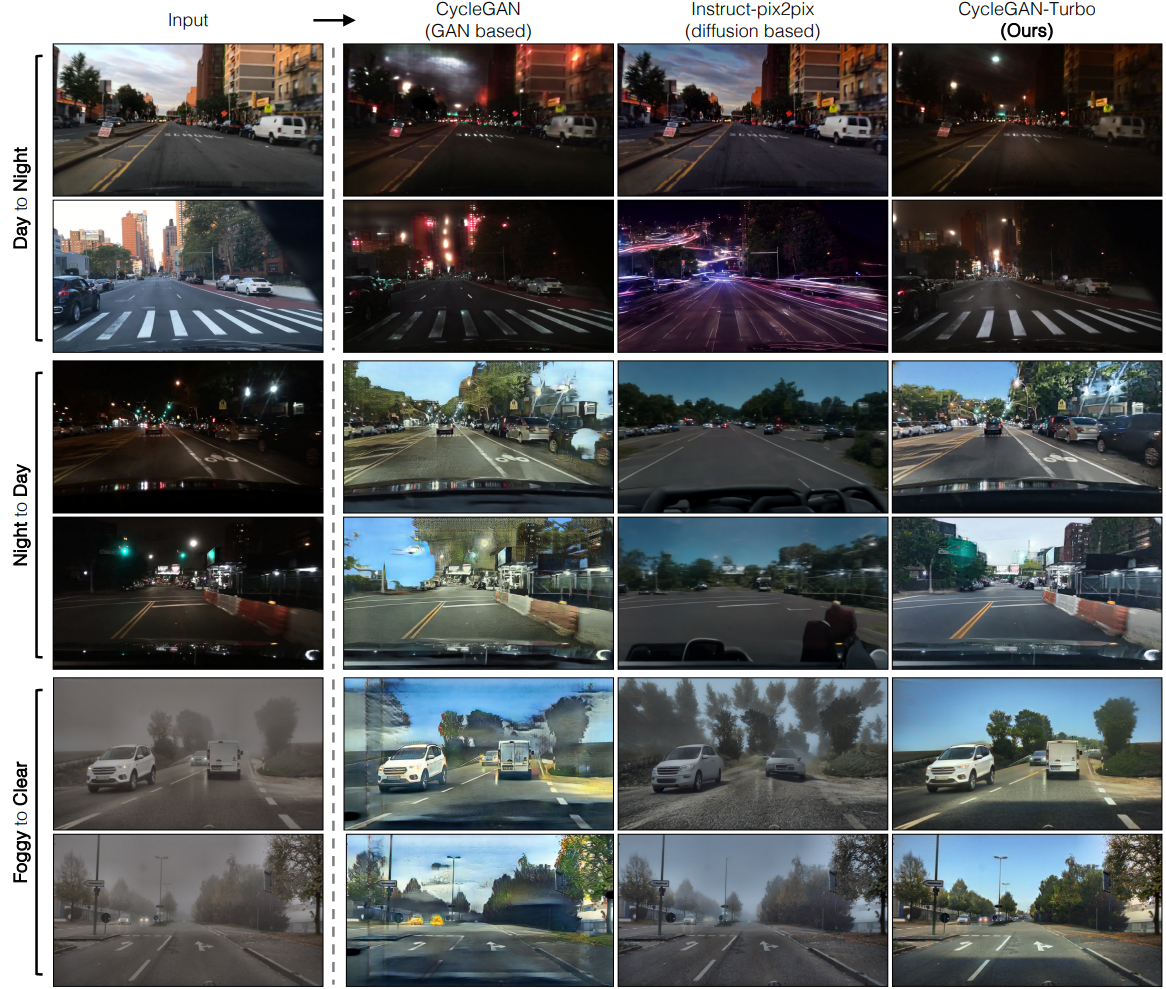
\includegraphics[width=0.5\linewidth]{images/day_night.png}
    
\end{figure}
\end{frame}





\begin{frame}
    \frametitle{Experiments - Paired Image Translation}
    \framesubtitle{Comparison to Unpaired Methods}

    \begin{table}
        \centering
    
        \resizebox{\linewidth}{!}{
        \begin{tabular}{l c cc cc cc cc}
            \toprule 
            \multirow{3}{*}{\textbf{Method}} 
            & \multirow{3}{*}{\textbf{\shortstack[c]{Infrence \\ time }}} 
            & \multicolumn{2}{c}{\textbf{Day $\rightarrow$ Night} }
            & \multicolumn{2}{c}{\textbf{Night $\rightarrow$ Day} }
            & \multicolumn{2}{c}{\textbf{Clear $\rightarrow$ Foggy} }
            & \multicolumn{2}{c}{\textbf{Foggy $\rightarrow$ Clear} }
            \\
    
            \cmidrule(lr){3-4} \cmidrule(lr){5-6} \cmidrule(lr){7-8} \cmidrule(lr){9-10} 
            &
            & \multirow{2}{*}{\shortstack[c]{FID $\downarrow$ }}  
            & \multirow{2}{*}{\shortstack[c]{DINO \\ Struct. $\downarrow$ }} 
    
            & \multirow{2}{*}{\shortstack[c]{FID $\downarrow$ }}  
            & \multirow{2}{*}{\shortstack[c]{DINO \\ Struct. $\downarrow$ }} 
    
            & \multirow{2}{*}{\shortstack[c]{FID $\downarrow$ }}  
            & \multirow{2}{*}{\shortstack[c]{DINO \\ Struct. $\downarrow$ }} 
    
            & \multirow{2}{*}{\shortstack[c]{FID $\downarrow$ }}  
            & \multirow{2}{*}{\shortstack[c]{DINO \\ Struct. $\downarrow$ }} 
            
            \\ \\
            \cmidrule(lr){1-10}
    
            CycleGAN \cite{zhu2020unpaired} & 0.02s
            & 36.3 & 3.6 
            & 92.3 & 4.9 
            & 153.3 & 3.6 
            & 177.3 & 3.9 
            \\
            
            CUT \cite{park2020contrastive} & 0.03s
            & 40.7 & 3.5 
            & 98.5 & 3.8
            & 152.6 & 3.4 
            & 163.9 & 4.8  \\
            
            \hdashline
    
            SDEdit \cite{meng2022sdedit} & 3.10s
            & 111.7 & 3.4 
            & 116.1 & 4.1 
            & 185.3 & 3.1
            & 209.8 & 4.7\\
    
            
            Plug\&Play \cite{tumanyan2022plugandplay} & 19.67s
            & 80.8 & 2.9 
            & 121.3 & \textbf{2.8} 
            & 179.6 & 3.6 
            & 193.5 & 3.5 \\
            
            Pix2Pix-Zero \cite{parmar2023zeroshot}  & 43.28s
            & 81.3 & 4.7 
            & 188.6 & 5.8
            & 209.3 & 5.5
            & 367.2 & 13.0
            \\
            
            Cycle-Diffusion \cite{cyclediffusion}  & 11.38s
            & 101.1 & 3.1 
            & 110.7 & 3.7 
            & 178.1 & 3.6 
            & 185.8 & 3.1\\
    
            DDIB \cite{su2022dual} & 11.93s
            & 172.6 & 9.1
            & 190.5 & 7.8 
            & 257.0 & 13.0 
            & 286.0 & 7.2  \\
    
            InstructPix2Pix \cite{brooks2023instructpix2pix} & 11.41s
            & 80.7 & \textbf{2.1} 
            & 89.4 & 6.2 
            & 170.8 & 7.6 
            & 233.9 & 4.8 
            \\
            \hdashline
    
            CycleGAN-Turbo & 0.29s
            & \textbf{31.3} & 3.0
            & \textbf{45.2} & 3.8 
            & \textbf{137.0} & \textbf{1.4}
            & \textbf{147.7} & \textbf{2.4} \\
    
            \bottomrule 
        \end{tabular}
        }
        \vspace{-18pt}
    
        \label{tab:cmp_driving_ds}
    \end{table}


\end{frame}


% ---------- Ablation Study ----------
\begin{frame}
\frametitle{Experiments - Paired Image Translation}
\framesubtitle{Ablation Study}


    \begin{table}   
        \centering
        \resizebox{\linewidth}{!}{
        \begin{tabular}{l c c c | cc cc cc cc}
            \toprule 
            \multirow{3}{*}{\textbf{Method} }
            & \multirow{3}{*}{\shortstack[c]{\textbf{Input} \\ \textbf{Type} }}  
            & \multirow{3}{*}{\shortstack[c]{\textbf{Skip} }}  
            & \multirow{3}{*}{\shortstack[c]{\textbf{Pre} \\ \textbf{-trained} }}  
            & \multicolumn{2}{c}{\textbf{Horse $\rightarrow$ Zebra} }
            & \multicolumn{2}{c}{\textbf{Zebra $\rightarrow$ Horse} }
            \\
    
            \cmidrule(lr){5-6} \cmidrule(lr){7-8} \cmidrule(lr){9-10} \cmidrule(lr){11-12} 
    
            &&&& \multirow{2}{*}{\shortstack[c]{FID $\downarrow$ }}  
            & \multirow{2}{*}{\shortstack[c]{DINO \\ Struct. $\downarrow$ }} 
    
            & \multirow{2}{*}{\shortstack[c]{FID $\downarrow$ }}  
            & \multirow{2}{*}{\shortstack[c]{DINO \\ Struct. $\downarrow$ }} 
            
            \\ \\
            \cmidrule(lr){1-12}
            Conf. A & Direct Input & x & x
            & 128.6 (+214\%)  & 5.2 (+148\%)
            & 167.1 (+31\%)  & 4.6 (+156\%)
            \\
            
            Conf. B & ControlNet & x & \checkmark 
            & 41.2 (+0\%)  & 7.3 (+248\%)
            & \textbf{99.4 (-22\%)}  & 8.6 (+378\%)\\
    
            Conf. C & T2I-Adapter & x & \checkmark 
            & 55.4 (+35\%)  & 4.7 (+124\%)
            & 135.4 (+6\%) & 4.8 (+167\%)\\
            
            
            Conf. D & Direct Input & x & \checkmark
            & \textbf{40.1 (-2\%)}  & 4.4 (+110\%)
            & 116.2 (-9\%) & 3.0 (+67\%) \\
            
            
            \hdashline
            Ours & Direct Input & \checkmark & \checkmark
            & 41.0 & \textbf{2.1}
            & 127.5 & \textbf{1.8}  \\
    
            \bottomrule 
        \end{tabular}
        }
    \vspace{-10pt}
        \label{tab:ablation_study}
    \end{table}
\end{frame}

\begin{frame}
    \frametitle{Experiments - Paired Image Translation}
    \framesubtitle{Ablation Study}
    \begin{figure}
        \centering
        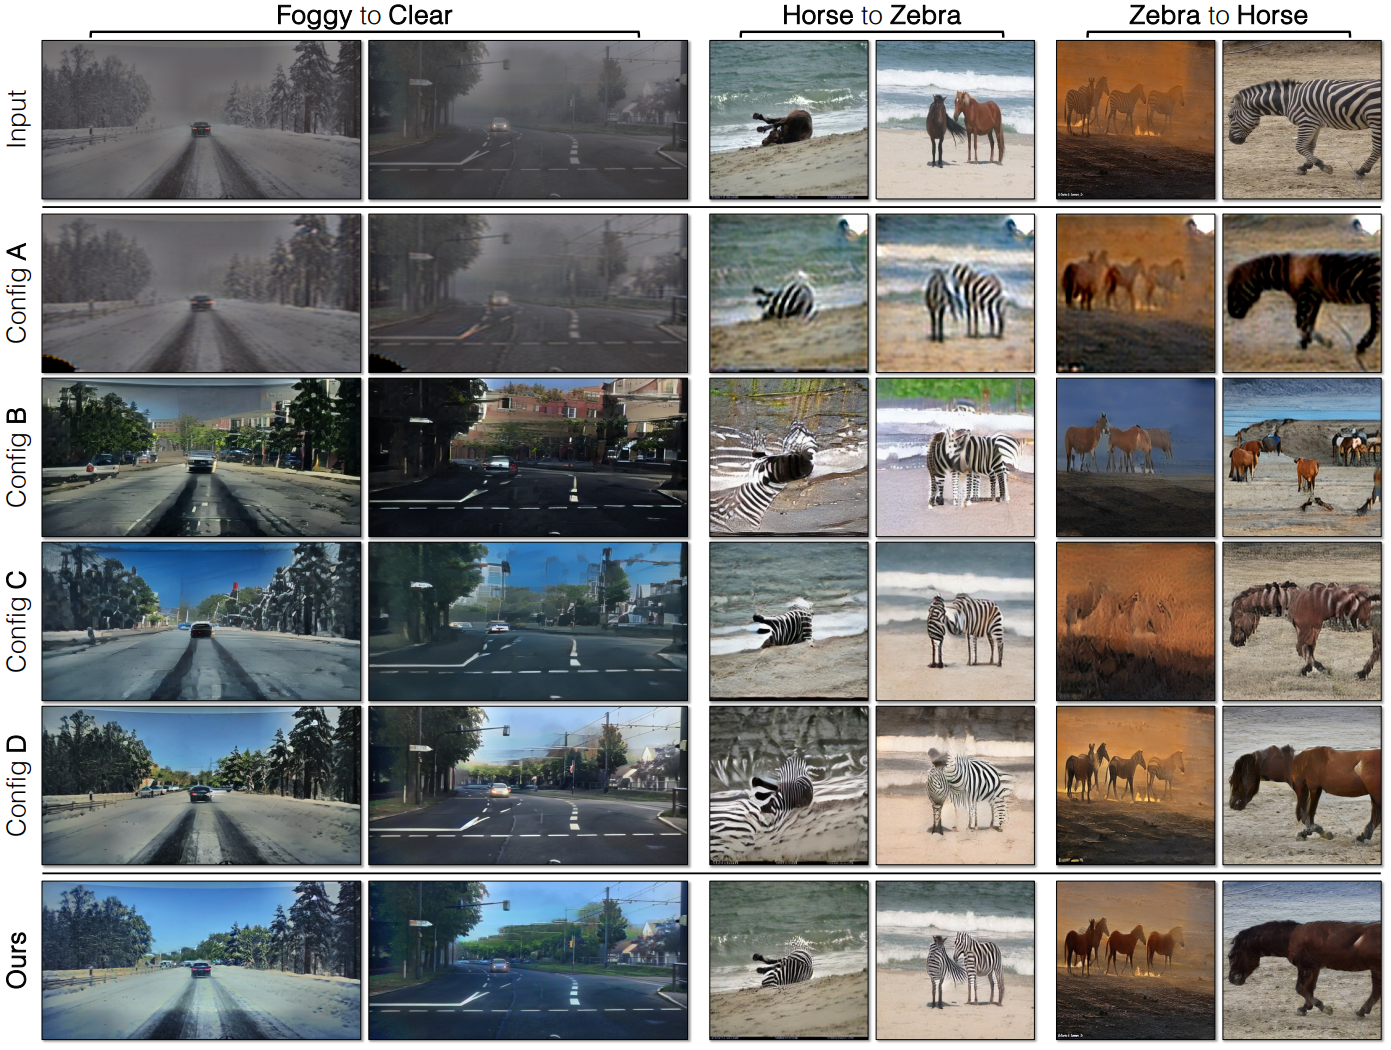
\includegraphics[width=0.55\linewidth]{images/ablation_images.png}
        
    \end{figure}
    \end{frame}
% ---------- Extensions ----------
\begin{frame}
\frametitle{Experiments - Unpaired Image Translation}
\framesubtitle{Training Details}
\begin{block}{Loss function}
    \begin{align}
        \arg \underset{G}{\min} \mathcal{L}_{\text{rec}} + \lambda _{\text{clip}} \mathcal{L}_{\text{CLIP}} + \lambda_{\text{GAN}}\mathcal{L}_{\text{GAN}}
    \end{align}
\end{block}
with $\mathcal{L}_{\text{rec}}$ = L2-Norm + LPIPS, $\lambda_{\text{clip}} = 4$ and $\lambda_{\text{GAN}} = 0.4$
\end{frame}

\begin{frame}
    \frametitle{Experiments - Unpaired Image Translation}
    \framesubtitle{Training Details}
        Edge-to-Image:
        \begin{itemize}
            \item Canny Edge Detector with random threshold
            \item Adam Optimizer with learning rate: 1e-5, batch size: 40, Steps: 7500
        \end{itemize}
        Sketch-to-Image:
        \begin{itemize}
            \item Synthetic sketches with multiple augmentations
            \item Initialized with Edge-to-Image model and fine-tuned for 5000 steps with same Optimizer
        \end{itemize}
\end{frame}

\begin{frame}
    \frametitle{Experiments - Unpaired Image Translation}
    \framesubtitle{Comparison to Unpaired Methods}
    \begin{figure}
        \centering
        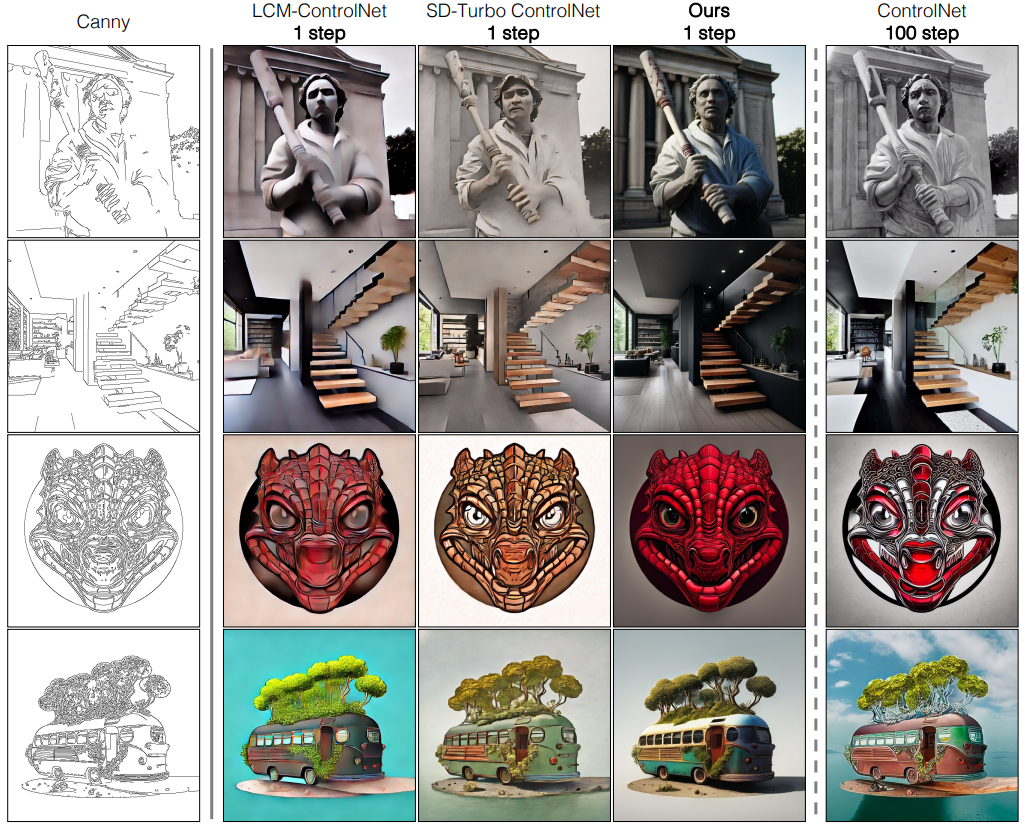
\includegraphics[width=0.5\linewidth]{images/unpaired_comp1.png}
        
    \end{figure}
\end{frame}

\begin{frame}
    \frametitle{Experiments - Unpaired Image Translation}
    \framesubtitle{Comparison to Unpaired Methods}
    \begin{figure}
        \centering
        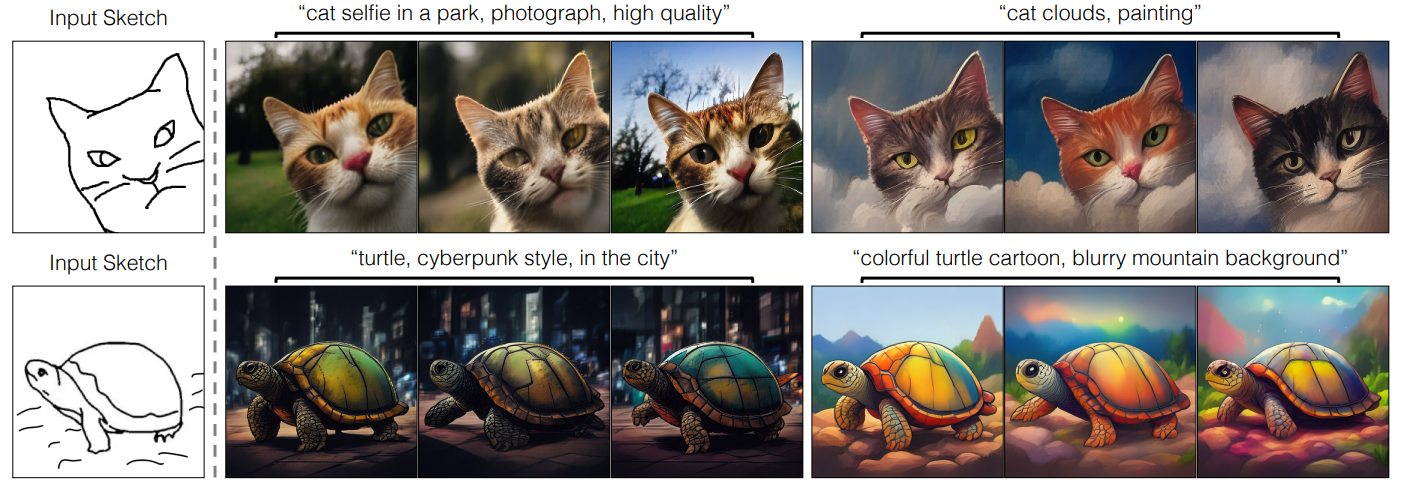
\includegraphics[width=1\linewidth]{images/unpaired_comp2.png}
            
    \end{figure}
\end{frame}
